% !TEX program = xelatex
\documentclass[11pt,a4paper]{article}

% ----------------------------------------------------------------------------------------
% Packages
% ----------------------------------------------------------------------------------------
\usepackage[top=1.5cm, bottom=1.5cm, left=2cm, right=2cm]{geometry} 
\usepackage{xeCJK}       % 支持中文
\usepackage{titlesec}    
\usepackage{enumitem}    
\usepackage{hyperref}    
\usepackage{xcolor}      
\usepackage{fontawesome5} 
\usepackage{calc}
\usepackage{graphicx} 
\usepackage{tikz}      

% ----------------------------------------------------------------------------------------
% Font Settings
% ----------------------------------------------------------------------------------------
\setCJKmainfont[BoldFont=FandolSong-Bold, ItalicFont=FandolKai-Regular]{FandolSong-Regular}
\setCJKsansfont[BoldFont=FandolHei-Bold]{FandolHei-Regular}
% 如果在本地 Windows 编译且没有 Fandol 字体，可注释掉上面两行，使用下面这行：
% \setCJKmainfont{SimSun} 

% ----------------------------------------------------------------------------------------
% Custom Formatting
% ----------------------------------------------------------------------------------------
\linespread{1.15} 

\titleformat{\section}
  {\Large\bfseries\raggedright} 
  {}{0em}                      
  {}                           
  [\titlerule]                 

\setlist[itemize]{leftmargin=*, parsep=0pt, itemsep=2pt, topsep=2pt}

% ----------------------------------------------------------------------------------------
% Document Start
% ----------------------------------------------------------------------------------------
\begin{document}

% ========================================================================================
% Header (Including Profile Picture)
% ========================================================================================
\noindent 
\begin{minipage}[t]{0.73\textwidth} 
    \vspace{0pt} 
    {\Huge\bfseries 朱昱泽} \\[0.6em] 
    {\large
    \faUniversity\ 中国科学院大学，中国北京，100049 \\[0.4em]
    \faEnvelope\ \href{mailto:zhuyuze23@mails.ucas.ac.cn}{zhuyuze23@mails.ucas.ac.cn} \quad | \quad
    \faPhone\ +86 155-5712-1756
    }
\end{minipage}%
\hfill 
\begin{minipage}[t]{0.23\textwidth} 
    \vspace{0pt} 
    \raggedleft 
    % Ensure the width is between 2.8cm and 3.0cm
    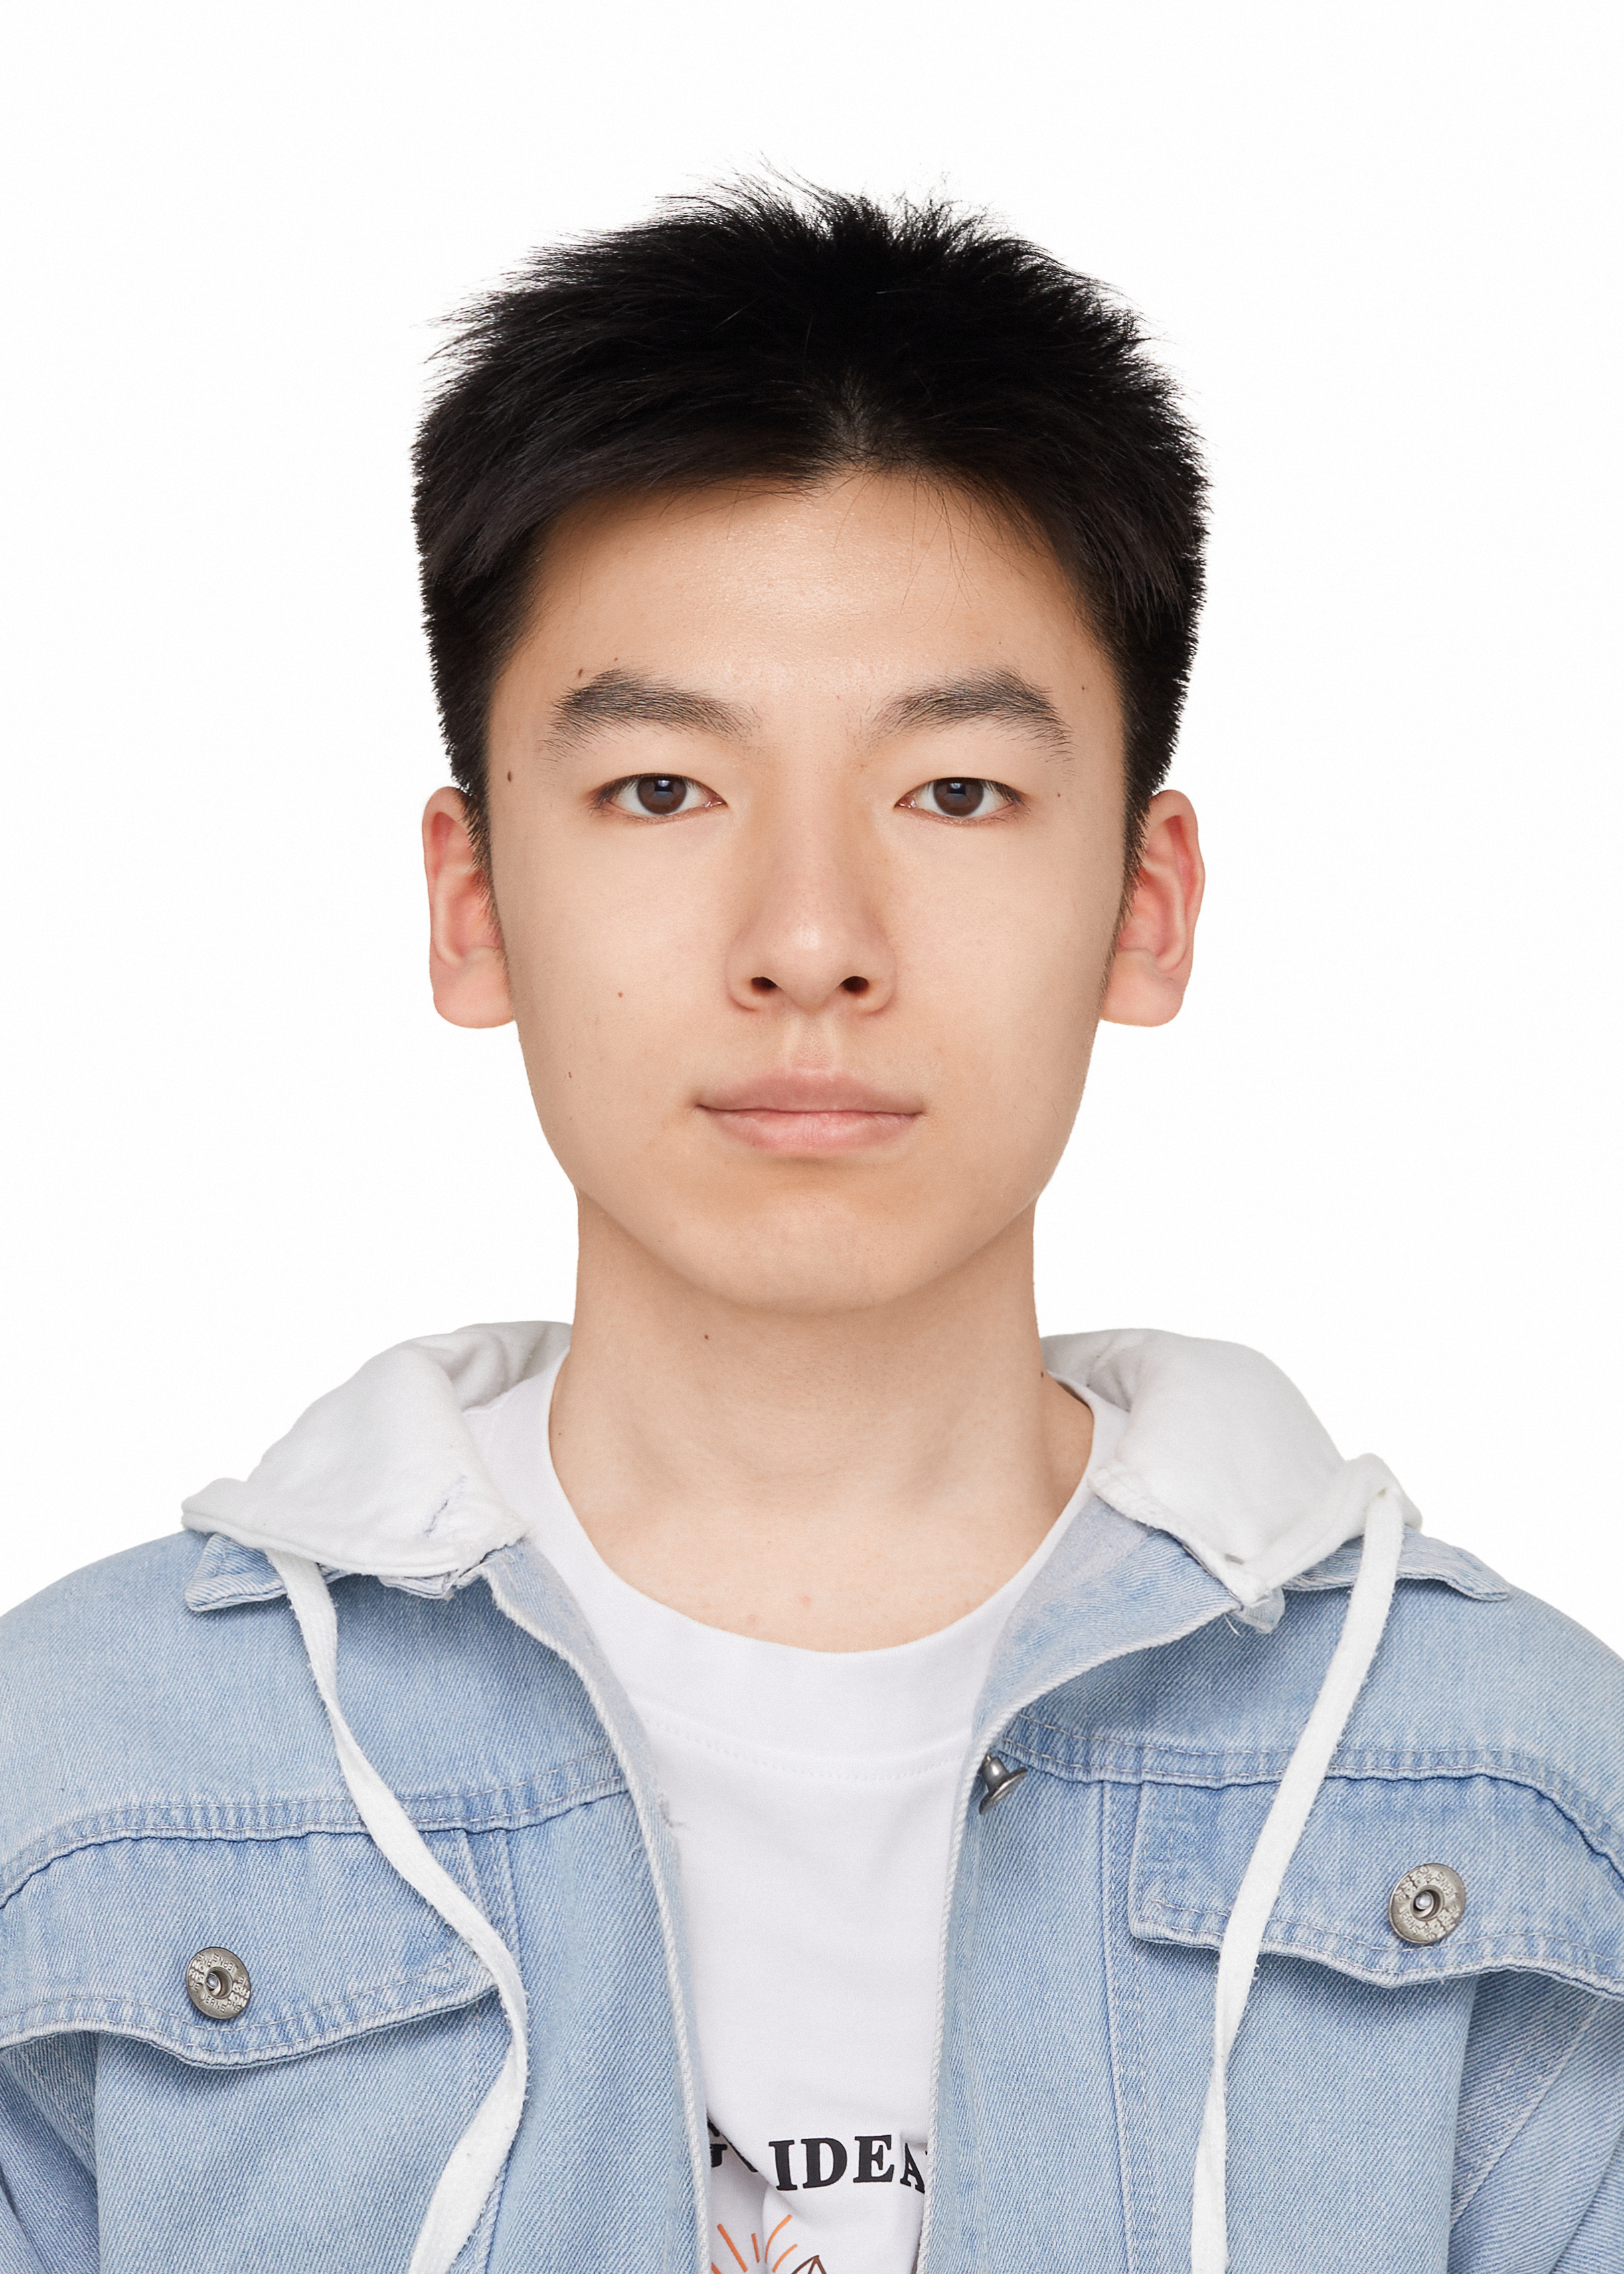
\includegraphics[width=2.8cm, keepaspectratio]{profile.jpg}
\end{minipage}

% ========================================================================================

% ----------------------------------------------------------------------------------------
% Education
% ----------------------------------------------------------------------------------------
\section{教育背景}
\textbf{中国科学院大学 (UCAS)} \hfill 中国北京 \\
\textit{工学学士，人工智能学院} \hfill 2023.09 -- 2027.07 (预计)
\begin{itemize}
    \item \textbf{GPA:} 3.87 / 4.0 \quad \textbf{排名:} 12/85 (前 15\%)
    \item \textbf{核心课程:} 计算机视觉、自然语言处理、机器人学（研讨课）、模式识别、数据结构等。
\end{itemize}

% ----------------------------------------------------------------------------------------
% Experience
% ----------------------------------------------------------------------------------------
\section{实习经历}
\textbf{中科第五纪 (FiveAges)} \hfill 具身智能算法研究实习生 \\
\textit{具身智能算法组，北京} \hfill 2026.03 -- 至今 \\
\textit{(导师：黄岩 研究员)}
\begin{itemize}
    \item \textbf{研究方向:} 具身智能算法研发，聚焦\textbf{视觉-语言-动作 (VLA)} 模型。
    \item \textbf{核心工作:} 参与 VLA 模型的算法研究与工程落地，致力于在真实机器人系统上部署并验证算法，推动学术研究与产业应用的衔接。
\end{itemize}

\vspace{0.4em}
\textbf{中国科学院自动化研究所 (CASIA)} \hfill 研究实习生 \\
\textit{多模态人工智能系统全国重点实验室，北京} \hfill 2025.07 -- 2026.01 \\
\textit{(导师：高君宇 副研究员 / 徐常胜 研究员)}
\begin{itemize}
    \item \textbf{研究方向:} 具身智能中的视觉语言导航 (VLN)，重点研究基于\textbf{自修正 (self-correction)} 的导航机制。
    \item \textbf{核心贡献:} 
    \begin{itemize}
        \item 构思创新方法并细化落地，提出了一种基于环境反馈的新型动态路径修正框架。
        \item 独立开发了\textbf{主实验代码库}，进行了详细的\textbf{数据分析}与\textbf{消融实验}，定量验证了各模块的贡献。
        \item 在 \textbf{R2R-CE} 和 \textbf{RxR-CE}（连续环境）数据集上进行了广泛的对比实验，证明所提方法有效提升了导航成功率。
    \end{itemize}
    \item \textbf{成果产出:} 作为第二作者合作撰写论文一篇，已投稿至顶级会议 ICML 2026（在审）。
\end{itemize}

% ----------------------------------------------------------------------------------------
% Publications
% ----------------------------------------------------------------------------------------
\section{论文发表}
\begin{itemize}
    \item Xuan Yao, \textbf{Yuze Zhu}, Junyu Gao, Zongmeng Wang, Changsheng Xu. ``\textit{[Title Anonymized for Double-Blind Review]}''. 
    \hfill \textbf{已投稿至 ICML 2026 (在审)}
    \item \textit{注：由于 ICML 双盲评审机制，论文具体题目暂未列出。}
\end{itemize}

% ----------------------------------------------------------------------------------------
% Course Project Experience
% ----------------------------------------------------------------------------------------
\section{课程项目经历}
\textbf{多模态测谎系统 (多媒体信息处理)} \hfill 核心开发者 \\
\textit{技术栈: Python, Qwen3-VL, WavLM, Transformer} \hfill 2025.10 -- 2025.12
\begin{itemize}
    \item 旨在通过分析面部微表情与语音特征实现高精度测谎。
    \item 利用 \textbf{Qwen3-VL} 大模型提取高维视觉与文本特征，并结合 \textbf{WavLM} 提取语音情感特征。
    \item 设计了多模态特征拼接网络与分类器，在测试集上实现了较高的识别准确率。
\end{itemize}

\textbf{基于 3D Residual U-Net 的 MRI 重建 (认知神经科学)} \hfill 算法设计与实现 \\
\textit{技术栈: PyTorch, 医学图像处理, 3D 卷积神经网络} \hfill 2025.11 -- 2025.12
\begin{itemize}
    \item 针对低场 MRI 图像信噪比低的问题，探索了基于深度学习的图像增强方法。
    \item 搭建并训练了 \textbf{3D Residual U-Net}，利用残差连接加速收敛并保留高频细节，成功实现了从低场到高场 MRI 的高质量重建。
\end{itemize}

\textbf{遥控机器人小车组装与控制 (机器人研讨课)} \hfill 独立完成 \\
\textit{技术栈: Arduino, Sensors, 控制原理} \hfill 2024.03 -- 2024.06
\begin{itemize}
    \item 领导了机器人小车的硬件选型与组装，并调试了电机驱动与传感器模块。
    \item 开发了控制程序以实现基础的避障与遥控巡航功能。
\end{itemize}

% ----------------------------------------------------------------------------------------
% Honors & Awards
% ----------------------------------------------------------------------------------------
\section{荣誉奖项}
\begin{itemize}
    \item \textbf{本科生优秀奖学金二等奖} (综合测评前 15\%) \hfill 2024
    \item \textbf{三好学生}，中国科学院大学 \hfill 2024
    \item \textbf{三好学生}，中国科学院大学 \hfill 2023
\end{itemize}

% ----------------------------------------------------------------------------------------
% Extracurricular Experience
% ----------------------------------------------------------------------------------------
\section{社会实践}
\textbf{“春分工程”科普志愿项目} \hfill 核心志愿者 \hfill 2023 -- 至今
\begin{itemize}
    \item \textbf{科普讲座:} 在北京十余所小学开展科普讲座，通过焰色反应演示激发学生的科学好奇心。
    \item \textbf{内容创作:} 参与撰写了“春分工程科学百科”的 \textbf{60 余个词条}，将复杂的概念转化为通俗易懂的文章。
\end{itemize}

% ----------------------------------------------------------------------------------------
% Skills & Languages
% ----------------------------------------------------------------------------------------
\section{技能与语言}
\begin{itemize}
    \item \textbf{编程语言:} Python (熟练), C/C++, LaTeX
    \item \textbf{框架与工具:} PyTorch, HuggingFace, Linux, Git, Docker
    \item \textbf{语言能力:} 中文 (母语), 英文 (TOEFL 5.0/6.0, 具备流利的学术读写能力)
\end{itemize}

\end{document}